\documentclass{article}
\usepackage[utf8]{inputenc}
\usepackage{gensymb}
\usepackage{graphicx}
\usepackage{parskip}
\usepackage{datetime}
\usepackage{amsmath, bm}

\newcommand{\HRule}{\rule{\linewidth}{0.5mm}}

\newdateformat{monthyear}{\monthname[\THEMONTH], \THEYEAR}

\begin{document}

\pagenumbering{gobble}

\begin{center}

\HRule \\[0.4cm]
{ \huge \bfseries Lab 2: INS and Kalman Filter \\[0.4cm] 
\Large \bfseries TTK5: Kalman Filtering and Navigation \\[0.4cm] } 

\HRule \\[1.5cm]

\begin{center} \large
\emph{By:}\\
\textbf{Andreas Nordby Vibeto}\\
andvibeto@gmail.com \\
(andreanv@stud.ntnu.no)
\end{center}

\vfill

{\large \monthyear\today}

\end{center}
\newpage
\pagenumbering{arabic}

\section*{Task 1}
\begin{figure}[!ht]
    \centering
    \makebox[\textwidth][c]{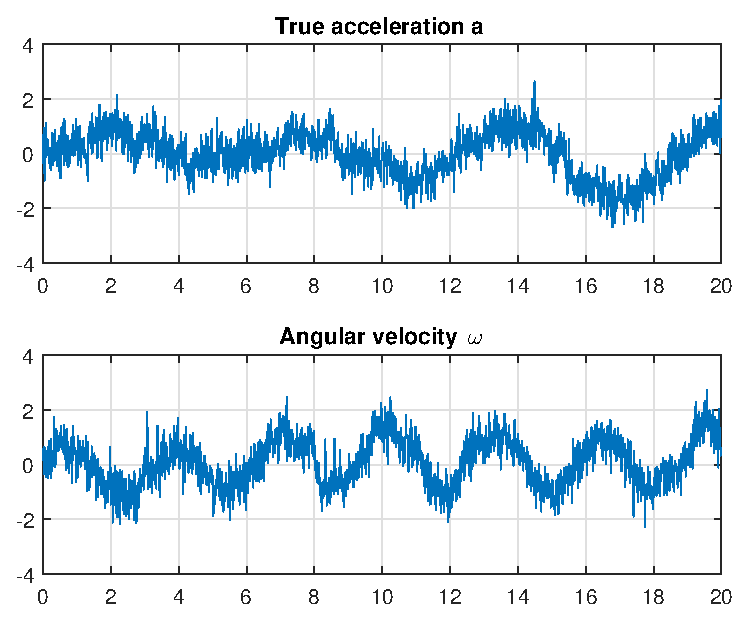
\includegraphics[width=1.25\textwidth, keepaspectratio=true]{../src/task1.eps}}
    \caption{True acceleration and angular velocity.}
\end{figure}

\section*{Task 2}
In order to discretize the system, it must first be written as a state space model. The system

\begin{subequations}
\begin{equation}
	\dot{x} = v 
\end{equation}
\begin{equation}
	\dot{v} = a
\end{equation}
\begin{equation}
	\dot{\theta} = \omega
\end{equation}
\end{subequations}

can be written as

\begin{subequations}
\begin{equation}
	\dot{\bm{x}} = \bm{A}\bm{x} + \bm{B}\bm{u}
\end{equation}
\begin{equation}
	\begin{bmatrix}
		\dot{x} \\ \dot{v} \\ \dot{\theta}
	\end{bmatrix}
	=
	\begin{bmatrix}
		0 & 1 & 0 \\
		0 & 0 & 0 \\
		0 & 0 & 0
	\end{bmatrix}
	\begin{bmatrix}
		x \\ v \\ \theta
	\end{bmatrix}
	+
	\begin{bmatrix}
		0 & 0 \\
		1 & 0 \\
		0 & 1
	\end{bmatrix}
	\begin{bmatrix}
		a \\ \omega
	\end{bmatrix}
	.
\end{equation}
\end{subequations}

By using forward Euler to discretize the system, it can be written on the form

\begin{equation}
	\bm{x}(t_{k+1}) = (\bm{I} + h\bm{A}(t_k)\bm{x}(t_k)) + h\bm{B}(t_k)\bm{u}(t_k)
\end{equation}

where $h$ is the step size. The discretized system then becomes

\begin{equation}
	\bm{x}(t_{k+1}) =
	\begin{bmatrix}
		1 & h & 0 \\
		0 & 1 & 0 \\
		0 & 0 & 1
	\end{bmatrix}
	\bm{x}(t_k) + 
	\begin{bmatrix}
		0 & 0 \\
		h & 0 \\
		0 & h
	\end{bmatrix}
	\bm{u}(t_k).
\end{equation}

Figure \ref{fig:disc_states} shows plots of the states in the discretized system.

\begin{figure}[!ht]
    \centering
    \makebox[\textwidth][c]{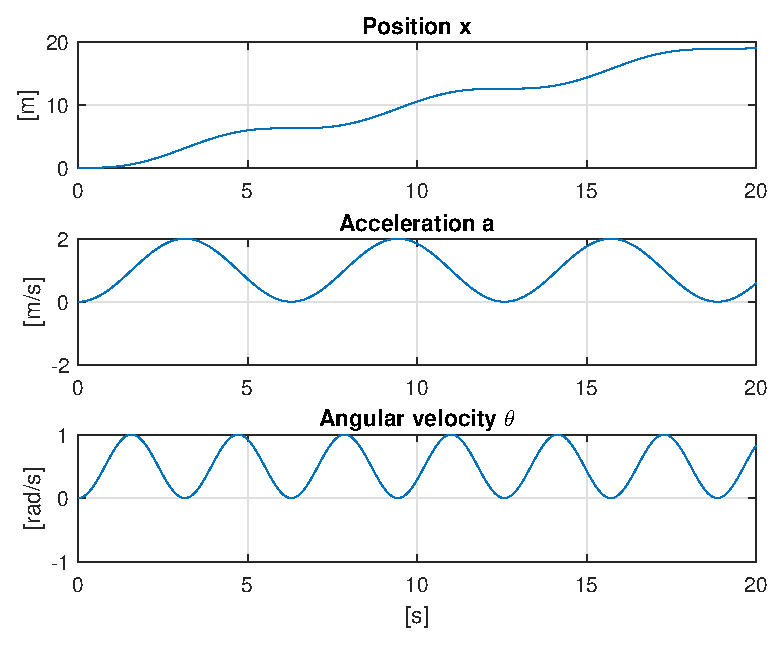
\includegraphics[width=1.25\textwidth, keepaspectratio=true]{../src/disc_states.eps}}
    \caption{States of the discretized system.}
    \label{fig:disc_states}
\end{figure}













\end{document}